\documentclass[a4paper, 12pt]{article}
\usepackage[total={17cm,25cm}, top=2.5cm, left=2.5cm, right=2.5cm,  includefoot]{geometry}
\usepackage[utf8]{inputenc}
\usepackage{array}
\usepackage{multirow}
\usepackage{hhline}
\usepackage{gensymb}
\usepackage{graphicx}
\graphicspath{ {} }
\usepackage[czech]{babel}
\usepackage{enumitem}
\usepackage{pdfpages}
\usepackage{amsmath}
\usepackage{verbatim}
\usepackage{listings}
\usepackage{hyperref}
\usepackage{amssymb}


\pagestyle{empty} % vypne číslování stránek




\usepackage[OT2,OT1]{fontenc}
\newcommand\cyr
{
\renewcommand\rmdefault{wncyr}
\renewcommand\sfdefault{wncyss}
\renewcommand\encodingdefault{OT2}
\normalfont
\selectfont
}
\DeclareTextFontCommand{\textcyr}{\cyr}
\def\cprime{\char"7E }
\def\cdprime{\char"7F }
\def\eoborotnoye{\char’013}
\def\Eoborotnoye{\char’003}
\setlength{\parindent}{1em} 
%\setlength{\parskip}{0.5ex}


\begin{document}

\begin{titlepage}
\begin{center}
\Huge
\vspace*{4.5cm}
Algoritmy v digitální kartografii\\
\vspace{0.2cm}

\Large  
Digitální model terénu a jeho analýzy\\
\vspace{0.2cm}

\normalsize  
Zimní semestr 2018/2019\\
%(oprava: 24. 11. 2018)
\vspace{14cm}
\end{center}

\begin{flushright}
\Large
Tereza Kulovaná \\
Markéta Pecenová \\
\end{flushright}

\end{titlepage}


\pagestyle{plain}     % zapne obyčejné číslování
\setcounter{page}{1}  % nastaví čítač stránek znovu od jedné

\tableofcontents
\newpage

\section{Zadání}
Zadání úlohy bylo staženo ze stránek předmětu \href{https://web.natur.cuni.cz/~bayertom/index.php/teaching/algoritmy-v-digitalni-kartografii}{155ADKG}.

\begin{figure}[h!]
	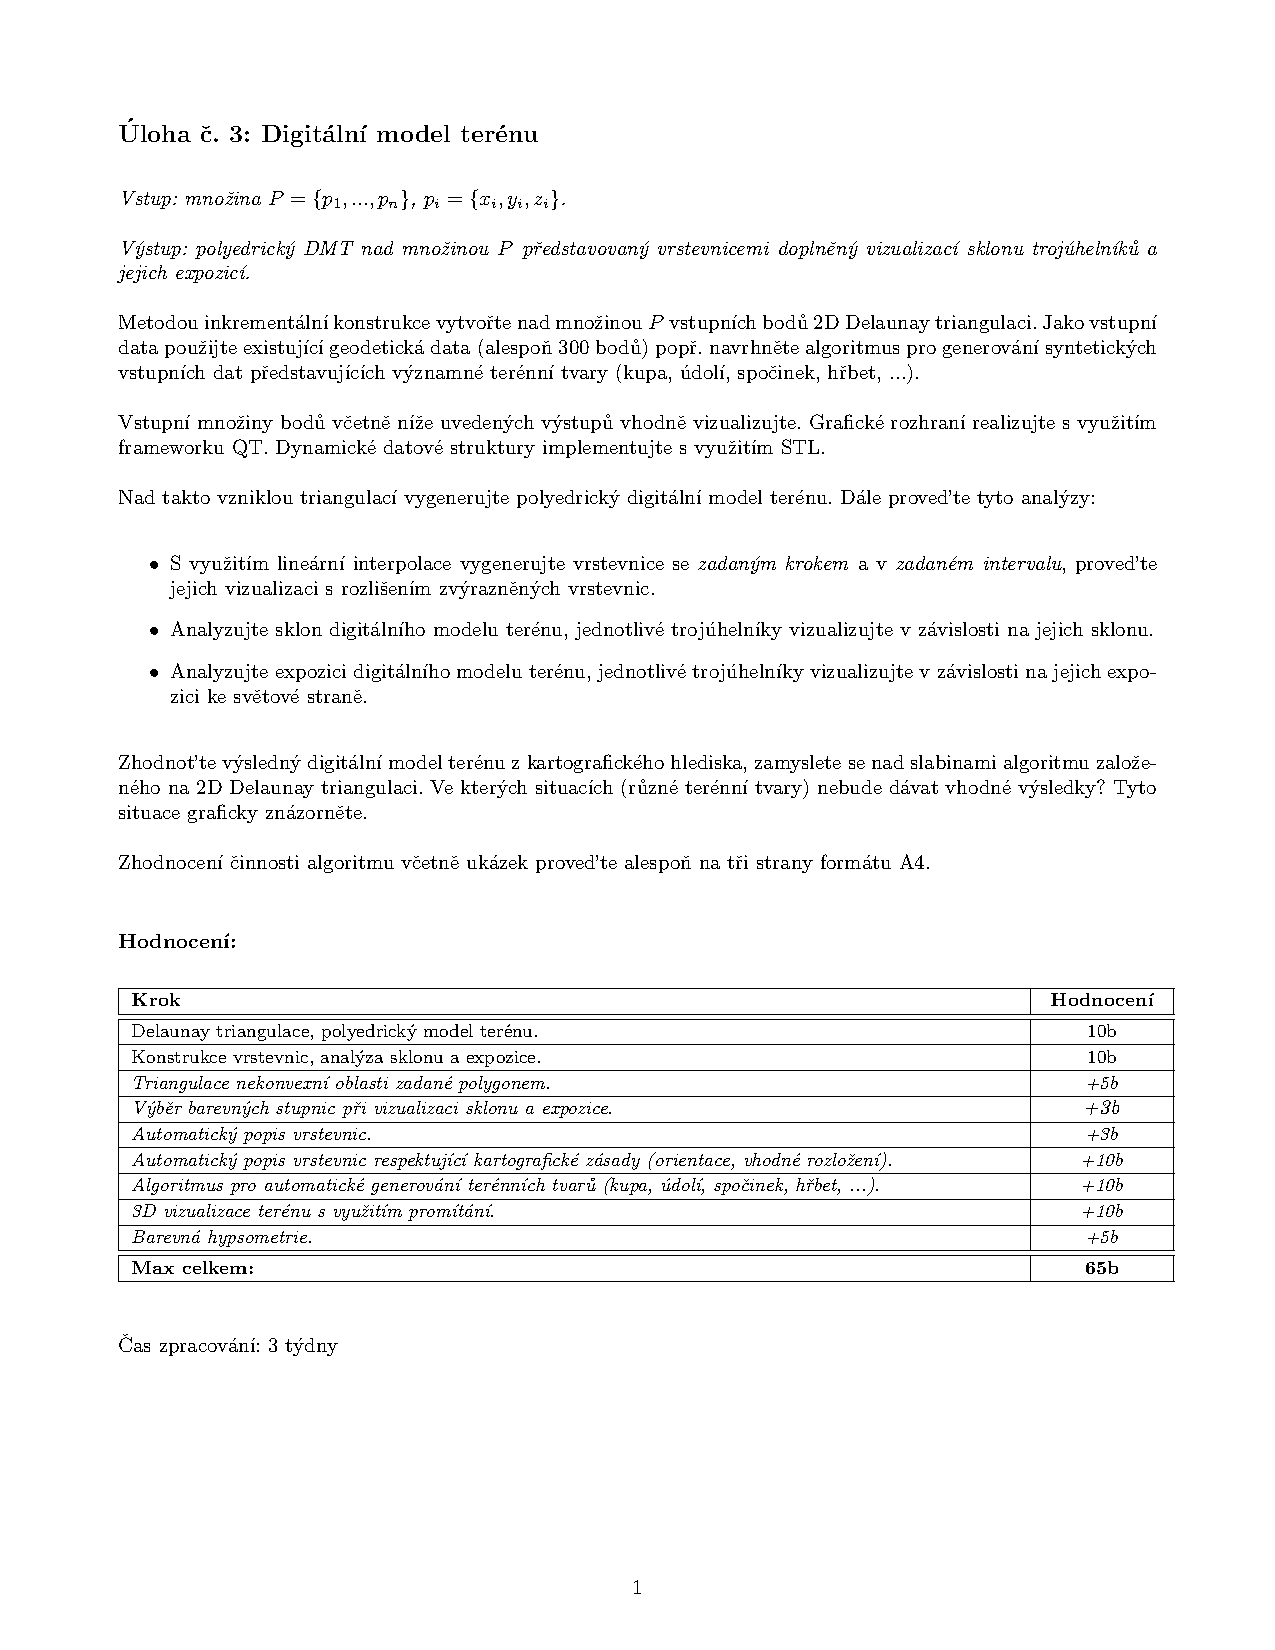
\includegraphics[clip, trim=0cm 4.5cm 0cm 3cm, width=1.0\textwidth]{./pictures/zadani03.pdf}
\end{figure}

V rámci této úlohy nebyly implementovány žádné bonusové úlohy.
\clearpage

\section{Popis a rozbor problému}
Úloha \textbf{Digitální model terénu a jeho analýzy} se zabývá vytvořením aplikace, která Delaunayovou triangulací nad vstupní množinou bodů $P$ vytvoří trojúhelníkovou síť, pro kterou se lineární interpolací vypočítají vrstevnice. Aplikace dále počítá a vhodně vizualizuje sklon a orientaci trojúhelníků ke světovým stranám.\\ 

Způsobů, jak geometricky zkonstruovat trojúhelníkovou síť, je více. Pro účely této úlohy byla vybrána Delaunayova triangulace, protože poskytuje optimální trojúhelníky z hlediska tvaru, což je zejména v kartografii velmi důležité. Delaunayova triangulace má čtyři základní vlastnosti:
\begin{enumerate}
\item Uvnitř kružnice opsané trojúhelníku $t_i \in DT$ neleží žádný jiný bod množiny $P$.
\item $DT$ maximalizuje minimální úhel v $\forall t_i$, avšak $DT$ neminimalizuje maximální úhel v $t_i$.
\item $DT$ je lokálně optimální i globálně optimální vůči kritériu minimálního úhlu.
\item $DT$ je jednoznačná, pokud žádné čtyři body neleží na kružnici.\footnote{Zdroj: \href{https://web.natur.cuni.cz/~bayertom/images/courses/Adk/adk5.pdf}{https://web.natur.cuni.cz}, slide 22}
\end{enumerate}
\vspace{0.4cm}

\section{Algoritmy}
Tato kapitola se zabývá popisem algoritmů, které byly v aplikaci implementovány. 

\subsection{Delanuayova triangulace}
Delaunyova triangulace byla realizována metodou inkrementální konstrukce, která je založena na postupném přidávání bodů do již vytvořené triangulace. Během výpočtu je používaná struktura $AEL$ (Active Edge List), která obsahuje všechny hrany, proto které ještě nebyl nalezen třetí bod trojúhelníku. Hrana, pro kterou byl bod nalezen, je vzápětí ze seznamu odstraněna. Před přidáním hran do seznamu je kontrolováno, zda se v něm již nenachází hrana s opačnou orientací. V takovém případě není hrana do seznamu přidána.\\

Mějme množinu bodů $P$ a orientovanou hranu $e_i$. Hledáme takový bod $p_i \in P$, který se nachází v levé polorovině vymezené hranou $e_i$, pro který dále platí, že poloměr kružnice jemu a hraně opsané je minimální. Během výpočtu jsou upřednostňovány body, jejichž středy opsaných kružnic se nachází v pravé polorovině. Je-li bod splňující výše uvedená kritéria nalezen, vytvoří se dvě nové orientované hrany $e_{i+1}$ a $e_{i+2}$, které se přidají do triangulace a do $AEL$. Původní hrana $e_i$ je z $AEL$ odstraněna. Není-li žádný vhodný bod nalezen, dochází k prohození orientace hrany $e_i$ a postup je opakován. Celý proces je ukončen ve chvíli, kde se v $AEL$ nenachází již žádná hrana. \\ 

Zjednodušený zápis algoritmu lze zapsat způsobem uvedeným níže:

\begin{enumerate}
\item Nalezení pivota $a$: $a$ = min($x$) a jemu nejbližší bod $b$
\item Vytvoření $e_1 = (a,b)$
\item Nalezení Delaunayova bodu: $r(k_i)$ = min, $k_i = (e_1,p_i)$
\item Podmínka: $p_i$ nenalezen $\rightarrow e_1 = (b,a)$, opakuj krok 3
\item Vytvoř zbylé hrany trojúhelníku: $e_2 = (b,p_i)$, $e_3 = (p_i,a)$
\item Přidej hrany do $AEL$: $AEL \leftarrow e_1$, $AEL \leftarrow e_2$, $AEL \leftarrow e_3$
\item Přidej hrany do triangulace $DT$: $DT \leftarrow e_1$, $DT \leftarrow e_2$, $DT \leftarrow e_3$
\item Dokud $AEL \neq \emptyset$:
\subitem Vezmi první hranu z $AEL \rightarrow e_1$
\subitem Prohoď orientaci: $e_1 = (b,a)$
\subitem Nalezení Delaunayova bodu: $r(k_i)$ = min, $k_i = (e_1,p_i)$
\subitem Podmínka: $p_i$ nalezen 
\subsubitem Vytvoř zbylé hrany trojúhelníku: $e_2 = (b,p_i)$, $e_3 = (p_i,a)$
\subsubitem Přidej hranu do $DT$: $DT \leftarrow e_1$
\subsubitem $add(e_2,AEL,DT), add(e_3,AEL,DT)$
\end{enumerate}
~\\
Lokální algoritmus $add$:
\begin{enumerate}
\item Prohoď orientaci: $e' = (b,a)$
\item Podmínka: $e' \in AEL \rightarrow$ odstraň $e'$ z $AEL$
\item Jinak: $AEL \leftarrow e$  
\item $DT \leftarrow e$
\end{enumerate}

\subsection{Vrstevnice}
Druhý algoritmus použitý v aplikaci slouží k výpočtu vrstevnic. Vrstevnice byly zkonstruovány metodou lineární interpolace, která je založena na předpokladu, že spád terénu mezi dvěma body $p_i$ se mění stejně, tedy konstantně. Výpočet byl proveden postupně pro všechny trojúhelníky a vrstevnice byly ukládány jako seznam hran.\\

Mějme trojúhelník $t_i$ tvořený třemi hranami $e_{1}(p_{1},p_{2})$, $e_{2}(p_{2},p_{3})$ a $e_{3}(p_{3},p_{1})$ a rovinu $\rho$ o výšce Z. Hledáme průsečnici roviny trojúhelníku $t_i$ s rovinou $\rho$. Pro kritérium $t=(z-z_i)(z-z_{i+1})$ mohou nastat tři základní situace:

\begin{enumerate}
\item $t > 0 \rightarrow e_i \notin \rho$ 
\item $t = 0 \rightarrow e_i \in \rho$
\item $t < 0 \rightarrow e_i \cap \rho$
\end{enumerate}
~\\
Pro případy 1 a 2 nebyly vrstevnice řešeny. Nastane-li případ 3 ($e_i \cap \rho$), je pro hranu $e_i$ a rovinu $\rho$ níže uvedenými vzorci vypočten průsečík $a$ o výšce $z_a$: (pro přehlednost uvedeno pro hranu $e_1$)

$$ x_a = \frac{(x_2-x_1)}{(z_2-z_1)}(z_a-z_1)+x_1 $$
$$ y_a = \frac{(y_2-y_1)}{(z_2-z_1)}(z_a-z_1)+y_1 $$

\subsection{Sklon}
Algoritmus pro výpočet sklonu počítá sklon jednotlivých trojúhelníků $t_i$. Sklon je úhel $\varphi$ mezi svislicí $n$ a normálou trojúhelníku $n_t$. Rovina trojúhelníku $t_i$ je určena vektory $u$, $v$. Sklon nabývá hodnot $\textless$0$^\circ$;90$^\circ\textgreater$ a v aplikaci je zobrazen v odstínech šedi.\\

$$n = (0,0,1)$$
$$n_t = \vec{u}\times \vec{v}$$
$$\varphi =\arccos\left(\frac{n_t \cdot n}{|n_t| |n|}\right)$$

\subsection{Orientace}
Orientace terénu $A$ je definována jako azimut průmětu gradientu normálového vektoru roviny trojúhelníku do roviny $x$,$y$. Nabývá hodnot $\textless$0$^\circ$;360$^\circ\textgreater$ a v aplikaci je zobrazen barevnou škálou.

$$n_t = \vec{u}\times \vec{v}$$
$$A = \arctan2\left(\frac{n_x}{n_y}\right)$$

%\section{Problematické situace}
%canvas -> transformace aby byla data vidět
%contours-> dostat se na celé číslo a od toho to počítat (nelze vzít nejmenší/největší hodnotu)

\section{Vstupní data}
Pro účely této úlohy byla použita data, která byla naměřena v rámci geodetické výuky v terénu v Mariánské u Jáchymova. Souřadnice X a Y byly pro tuto úlohu zredukovány na rozumnou velikost, souřadnice Z byla zachována. Body byly zaměřeny metodou GNSS a totální stanicí a znázorňují tamní louku a část silnice. Seznam vstupních bodů je uložen v textovém souboru testing\_data.txt. Soubor je nutné do aplikace nahrát pomocí tlačítka \textsl{Load points}. Struktura textového souboru je následující:\\

\noindent
\textit{Sloupec 1}: souřadnice X [m]\\
\textit{Sloupec 2}: souřadnice Y [m]\\
\textit{Sloupec 3}: souřadnice Z [m]\\

Po úspěšném/neúspěšném nahrání souboru je uživatel upozorněn hláškou. Uživatel nemůže kliknout na žádné jiné tlačítko pro výpočty, nejsou-li nahrána data (tlačítka jsou zašedivělá). Aplikace dále nedovoluje spustit výpočty, jejichž fungování je závislé na vygenerované trojúhelníkové síti, nebyla-li předtím vytvořena. Uživatel má dále možnost zvolit krok, v jakém se budou vykreslovat vrstevnice. Hodnoty lze měnit šipkami nahoru/dolů po 5 m nebo ručně vepsat hodnotu celého čísla v rozmezí 1 m až 100 m. Delaunayova triangulace, vrstevnice, sklon a orientace se generují stisknutím příslušných tlačítek.

\section{Výstupní data}
Vstupní množina bodů a nad ní vygenerovaná trojúhelníková síť je zobrazena ve grafickém okně aplikace. Vykreslování vrstevnic, sklonu a orientace je odděleno. U vrstevnic je každá pátá (hlavní) zvýrazněna. Sklon je v odstínech šedi (čím vyšší sklon, tím tmavší barva). Pro zobrazení orientace trojúhelníků ke světovým stranám byla využita prostřední kružnice barvené škály ze stránek společnosti \textit{ESRI}, viz níže. Aplikace je uvedena do výchozího stavu stisknutím tlačítka \textsl{Clear}.\\

\begin{figure}[h!]
	\centering
	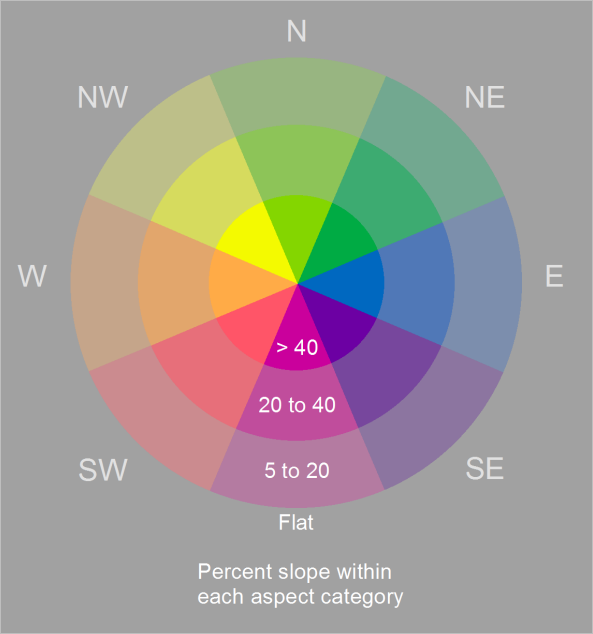
\includegraphics[width=8cm]{./pictures/skala.png}
	\caption{Barevná škála orientace trojúhelníků ke světovým stranám \href{https://www.esri.com/arcgis-blog/products/arcgis-pro/imagery/new-aspect-slope-raster-function-now-available/?fbclid=IwAR0LX-HblA_iPSqg19aUKDW096LjaShp9r_ql8QwA_OJ26EkcFTpOEWJrlg}{[Zdroj]}}
\end{figure}

\clearpage
\section{Aplikace}
V následují kapitole je představen vizuální vzhled vytvořené aplikace tak, jak ji vidí prostý uživatel.

\begin{figure}[h!]
	\centering
	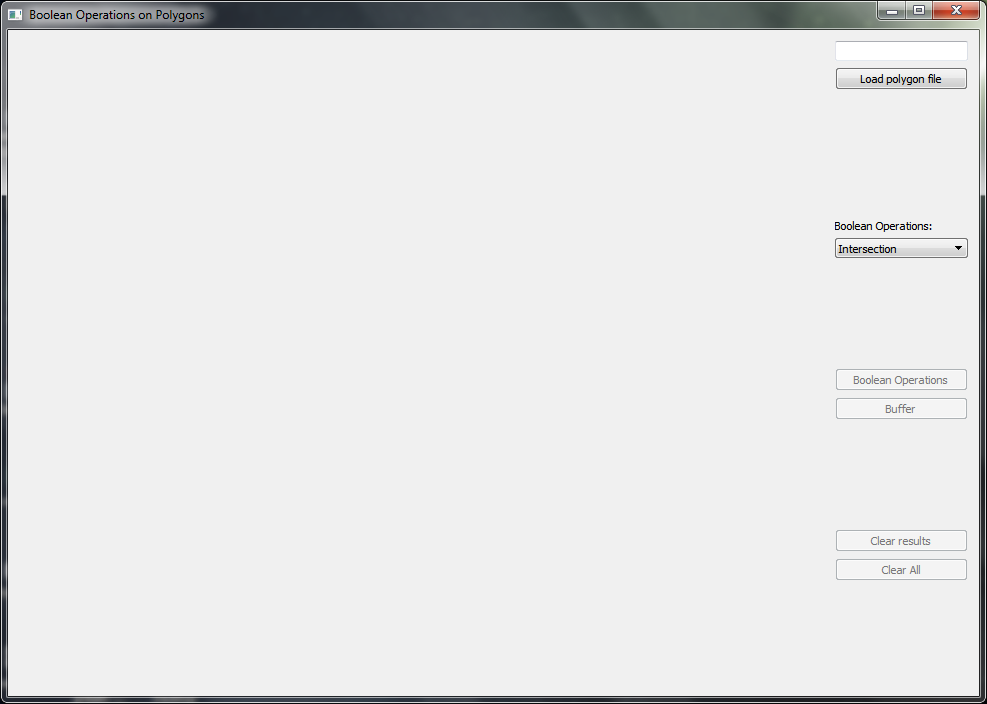
\includegraphics[width=14cm]{./pictures/app_default.png}
	\caption{Výchozí vzhled aplikace po spuštění}
\end{figure}

\begin{figure}[h!]
	\centering
	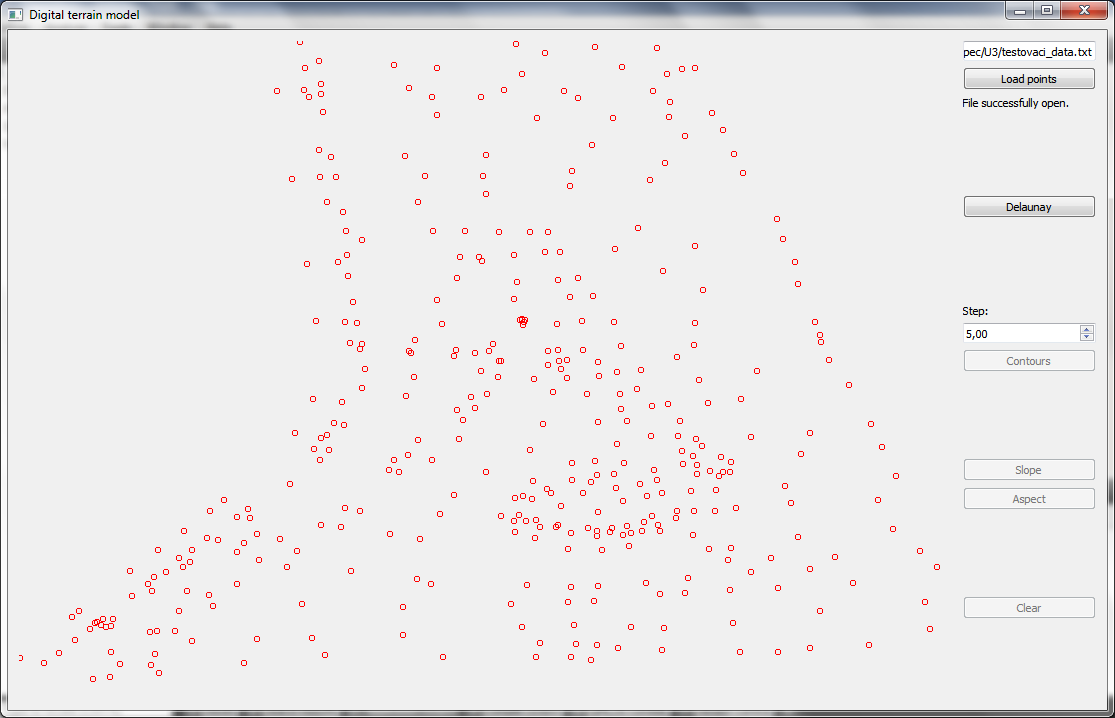
\includegraphics[width=14cm]{./pictures/app_load_points.png}
	\caption{Aplikace po nahrání vstupních dat}
\end{figure}

\begin{figure}[h!]
	\centering
	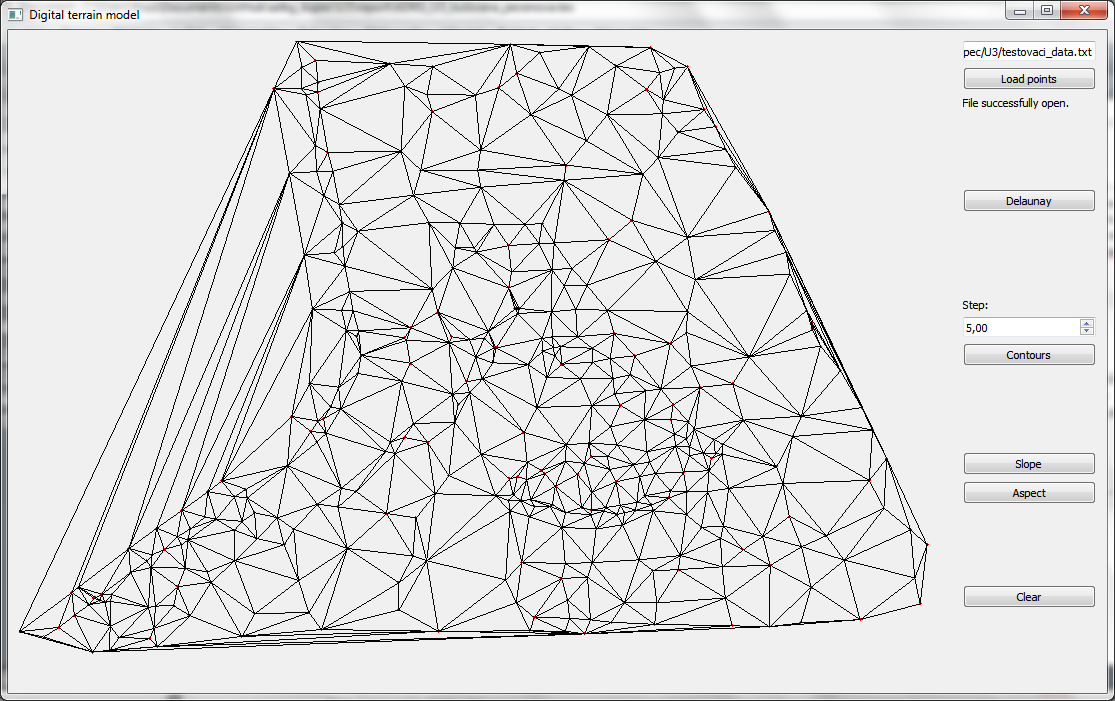
\includegraphics[width=15cm]{./pictures/app_delaunay.png}
	\caption{Trojúhelníková síť}
\end{figure}

\begin{figure}[h!]
	\centering
	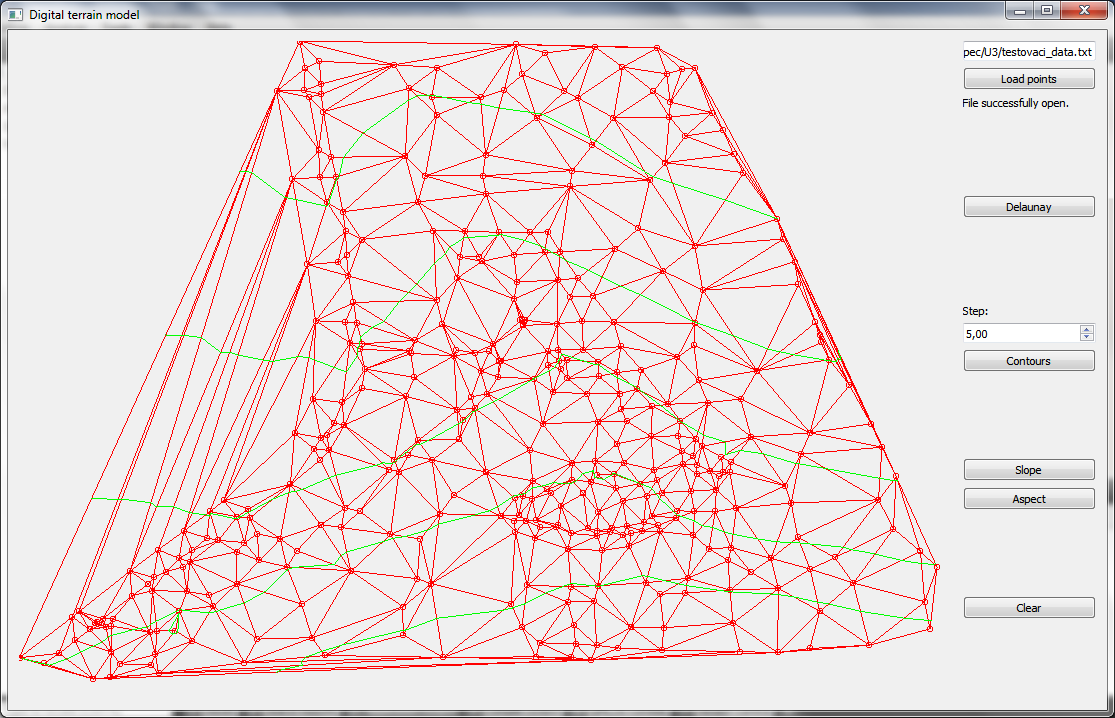
\includegraphics[width=15cm]{./pictures/app_contours.png}
	\caption{Vykreslení vrstevnic}
\end{figure}

\begin{figure}[h!]
	\centering
	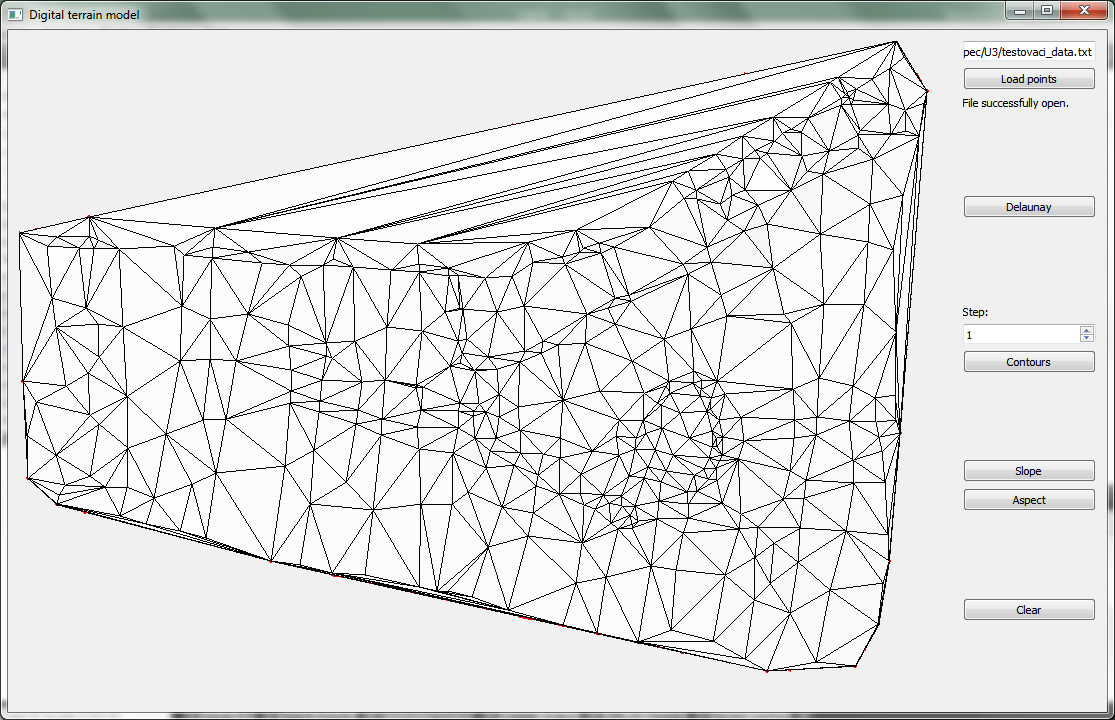
\includegraphics[width=15cm]{./pictures/app_slope.png}
	\caption{Sklon trojúhelníků}
\end{figure}

\begin{figure}[h!]
	\centering
	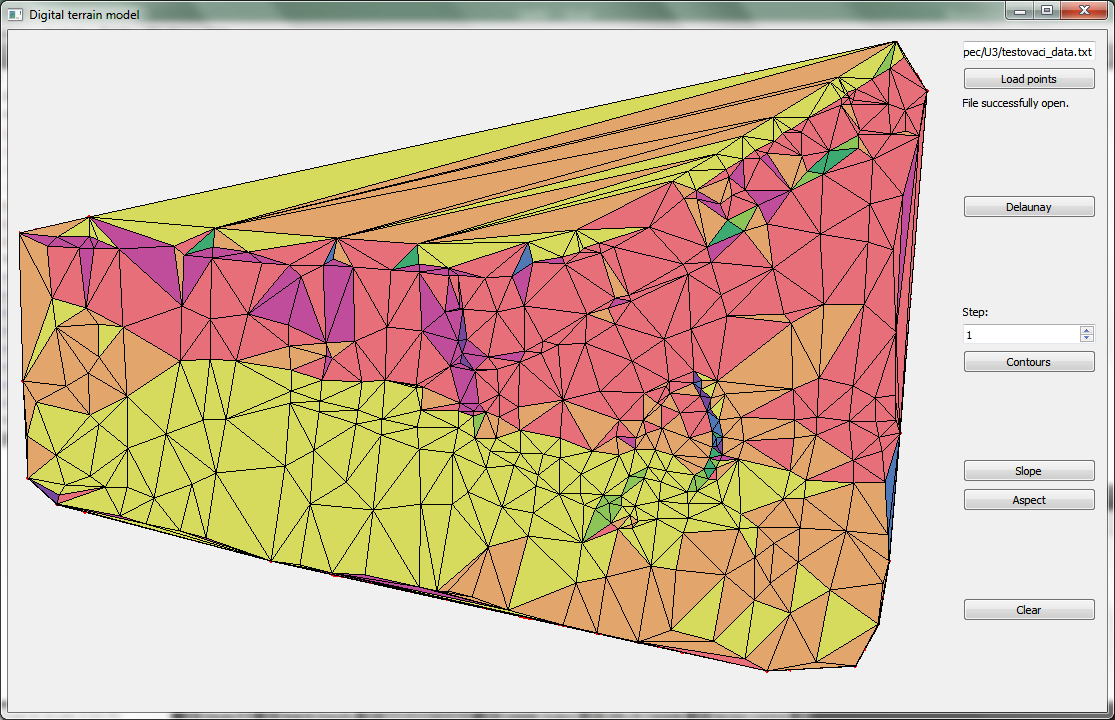
\includegraphics[width=15cm]{./pictures/app_aspect.png}
	\caption{Orientace trojúhelníků}
\end{figure}
\clearpage

\section{Zhodnocení činnosti algoritmu}
V následující kapitole je porovnán DMT z aplikace a DMT, který byl již dříve vyhotoven v SW \textit{Atlas}. Aplikace nezvládá zobrazovat současně vykreslené vrstevnice a sklon trojúhelníků. Ukázka výstupů je rozdělena do dvou snímků. 

\subsection{Celý model}
\begin{figure}[h!]
	\centering
	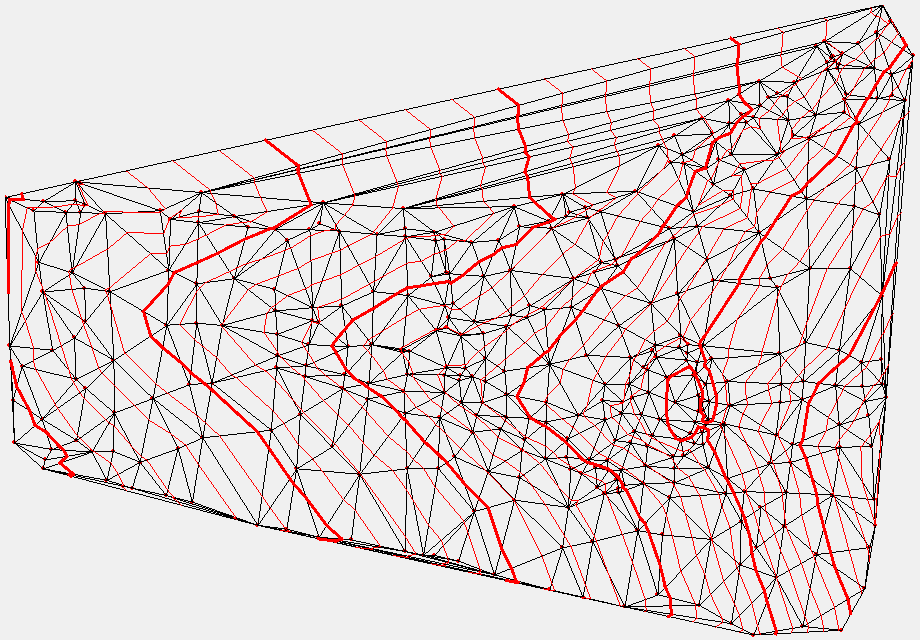
\includegraphics[width=12cm]{./pictures/kupec_dtm_contours.png}
	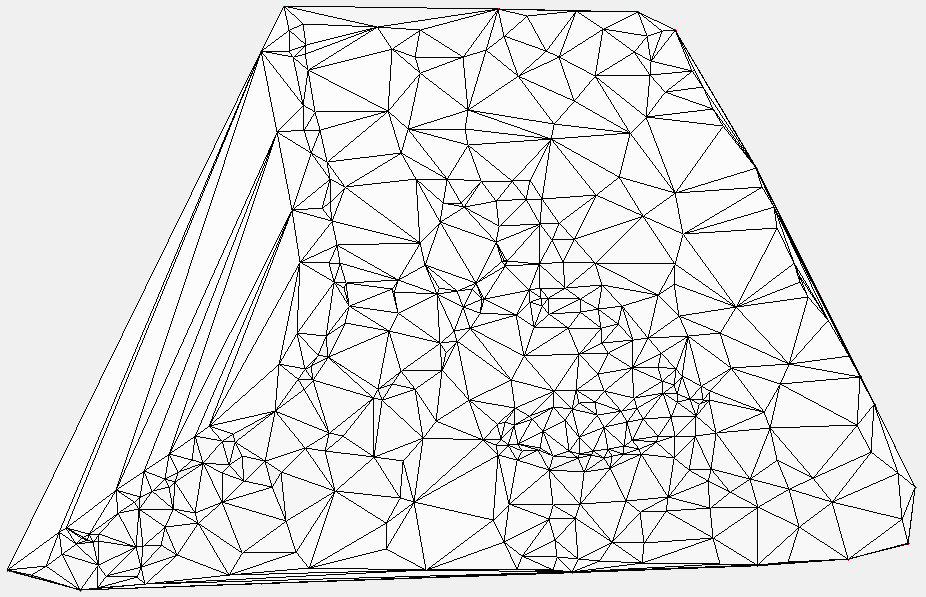
\includegraphics[width=12cm]{./pictures/kupec_dtm_slope.png}
	\caption{DMT vytvořený aplikací}
\end{figure}
\clearpage

\begin{figure}[h!]
	\centering
	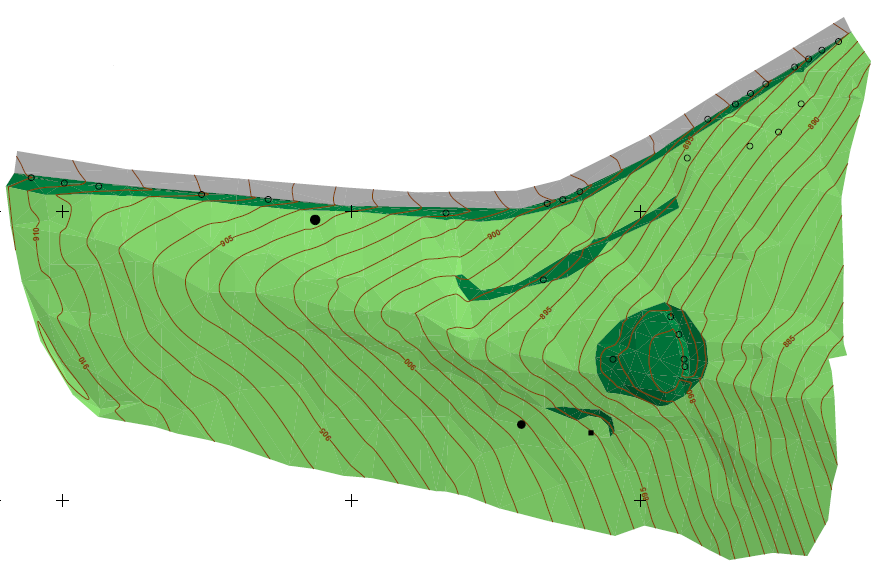
\includegraphics[width=13cm]{./pictures/atlas_dtm.png}
	\caption{DMT ze SW \textit{Atlas}}
\end{figure}

Na první pohled je patrné, že DMT ze SW \textit{Atlas} je kvalitněji vyhotoven. Problémem  Delaunayovy triangulace implementované v aplikaci je zejména chybějící možnost nadefinovat lomové a povinné hrany pro triangulaci. V horní části modelu podél silnice se vygenerovaly štíhlé trojúhelníky, které by správně vůbec neměly existovat, jelikož se nachází mimo zájmovou oblast. Vrstevnice z \textit{Atlasu} jsou vyhlazenější, neboť to bylo během generování modelu zajištěno funkcí pro vyhlazení vrstevnic, a vytvořená aplikace toto neumožňuje. Jelikož sklon terénu byl víceméně rovnoměrný, sklon generovaný v aplikaci není příliš viditelný. 

\subsection{Plošina}
\begin{figure}[h!]
	\centering
	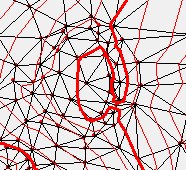
\includegraphics[width=7cm]{./pictures/kupec_plateau_contours.png}
	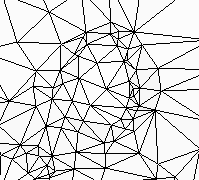
\includegraphics[width=7cm]{./pictures/kupec_plateau_slope.png}
	\caption{Plošina vytvořená aplikací}
\end{figure}

\begin{figure}[h!]
	\centering
	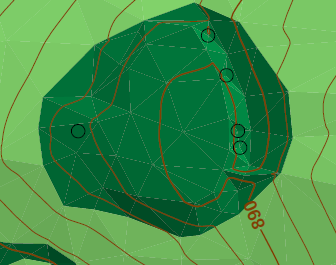
\includegraphics[width=7cm]{./pictures/atlas_plateau.png}
	\caption{Plošina ze SW \textit{Atlas}}
\end{figure}

Plošina uprostřed území je rozeznatelná zejména z tvarů vrstevnic. Z trojúhelníkové sítě je patrné, že je trochu vyvýšená, ale i tak to chce trochu představivosti.

\subsection{Hrana}
\begin{figure}[h!]
	\centering
	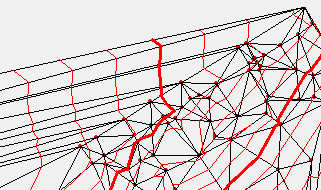
\includegraphics[width=7cm]{./pictures/kupec_edge_contours.png}
	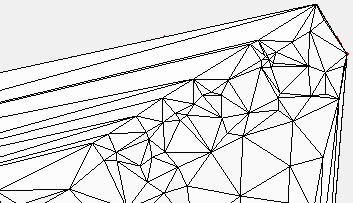
\includegraphics[width=7cm]{./pictures/kupec_edge_slope.png}
	\caption{Hrana silnice vytvořená aplikací}
\end{figure}

\begin{figure}[h!]
	\centering
	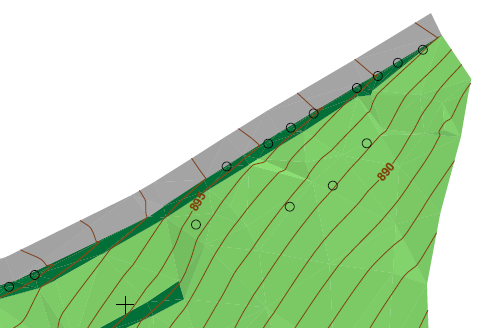
\includegraphics[width=10cm]{./pictures/atlas_edge.png}
	\caption{Hrana silnice ze SW \textit{Atlas}}
\end{figure}

Vygenerované vrstevnice v okolí silnice působí silně kostrbatým dojmem, avšak trojúhelníková síť poměrně věrně kopíruje tvar silnice. Jak již bylo zmíněno výše, velkým problémem jsou štíhlé trojúhelníky v horní části modelu, které by neměly existovat.


\subsection{Údolnice}
\begin{figure}[h!]
	\centering
	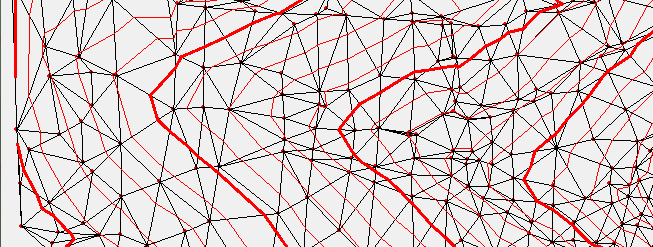
\includegraphics[width=7.5cm]{./pictures/kupec_thalweg_contours.png}
	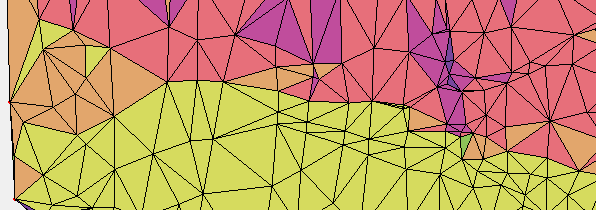
\includegraphics[width=7.5cm]{./pictures/kupec_thalweg_aspect.png}
	\caption{Údolnice vytvořená aplikací}
\end{figure}

\begin{figure}[h!]
	\centering
	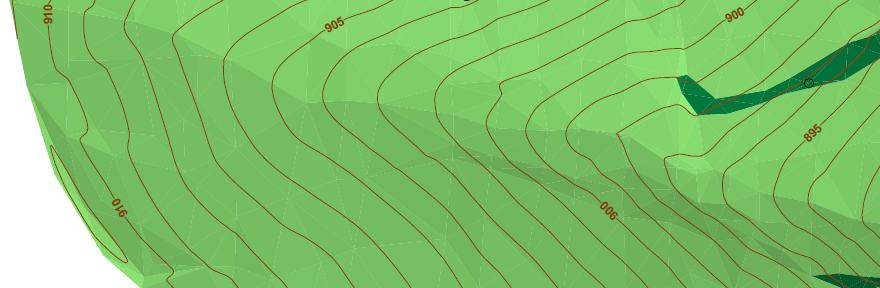
\includegraphics[width=15cm]{./pictures/atlas_thalweg.png}
	\caption{Údolnice ze SW \textit{Atlas}}
\end{figure}

Pro názornost porovnání byla tentokrát použita orientace trojúhelníků ke světovým stranám. Z jejich natočení je patrné, že ve středu dochází ke zlomu v terénním tvaru. Vrstevnice tento úkaz hezky vystihují. Ze všech částí DMT vystihla aplikace tento tvar v porovnání s DMT z \textit{Atlasu} nejvěrněji.
\clearpage
 
\section{Dokumentace}
Tato kapitola obsahuje dokumentaci k jednotlivým třídám.

\subsection{Algorithms}
Třída \textit{Algorithms} obsahuje metody pro výpočet Delaunayovy triangulace a analýzu DTM.

\subsubsection*{delaunayTriangulation}
Metoda \textbf{delaunayTriangulation} vytváří nad množinou bodů Delaunayovu triangulaci. Na vstupu je vektor bodů typu \texttt{QPoint3D}, metoda vrací uspořádaný vektor hran \texttt{Edge}, které tvoří jednotlivé trojúhelníky.\\

\textbf{Input}:
\begin{itemize}
\item \textsl{vector} $\textless$\texttt{QPoint3D}$\textgreater$ $points$
\end{itemize}

\textbf{Output}:
\begin{itemize}
\item \textsl{vector} $\textless$\texttt{Edge}$\textgreater$
\end{itemize}

\subsubsection*{createContours}
Metoda \textbf{createContours} vytváří nad vstupní množinou hran vrstevnice dle zadaného kroku, po kterém se vrstevnice budou vykreslovat.  Metoda vrací vektor hran, které představují vrstevnice.\\

\textbf{Input}:
\begin{itemize}
\item \textsl{vector} $\textless$\texttt{Edge}$\textgreater$ $dt$
\item \texttt{double} $z\_min$ $\rightarrow$ minimální výška
\item \texttt{double} $z\_max$ $\rightarrow$ maximální výška
\item \texttt{double} $dz$ $\rightarrow$ krok vrstevnic
\end{itemize}

\textbf{Output}:
\begin{itemize}
\item \textsl{vector} $\textless$\texttt{Edge}$\textgreater$
\end{itemize}

\subsection*{getSlope}
Metoda \textbf{getSlope} počítá sklon trojúhelníku, který je tvořen třemi body. Návratová hodnota typu \texttt{double} nabývá hodnot $\textless$0$^\circ$;90$^\circ\textgreater$ a vrací sklon trojúhelníku.\\

\textbf{Input}:
\begin{itemize}
\item \texttt{QPoint3D} $p_1$
\item \texttt{QPoint3D} $p_2$
\item \texttt{QPoint3D} $p_3$
\end{itemize}

\subsubsection*{getAspect}
Metoda \textbf{getAspect} počítá orientaci trojúhelníku, který je tvořen třemi body, ke světovým stranám. Návratová hodnota typu \texttt{double} vrací orientaci trojúhelníku ve stupních. Orientace je pravotočivá a nabývá hodnot $\textless$-180$^\circ$;180$^\circ\textgreater$.\\

\textbf{Input}:
\begin{itemize}
\item \texttt{QPoint3D} $p_1$
\item \texttt{QPoint3D} $p_2$
\item \texttt{QPoint3D} $p_3$
\end{itemize}

\subsubsection*{analyzeDTM}
Metoda \textbf{analyzeDTM} vytváří z vektoru hran trojúhelníky a počítá pro ně sklon a orientaci. Vypočtené hodnoty ukládá do datového typu \texttt{Triangle}. Návratová hodnota metody je vektor trojúhelníků typu \texttt{Triangle}.\\

\textbf{Input}:
\begin{itemize}
\item \textsl{vector} $\textless$\texttt{Edge}$\textgreater$ $dt$
\end{itemize}

\textbf{Output}:
\begin{itemize}
\item \textsl{vector} $\textless$\texttt{Triangle}$\textgreater$
\end{itemize}

\subsubsection*{getPointLinePosition}
Metoda \textbf{getPointLinePosition} určuje polohu bodu $q$ vzhledem k přímce tvořené dvěma body. Na vstupu jsou 3 body typu \texttt{QPoint3D}, návratová hodnota je nově definovaný typ \texttt{TPosition}.\\

\textbf{Input}:
\begin{itemize}
\item \texttt{QPoint3D} $q$
\item \texttt{QPoint3D} $a$
\item \texttt{QPoint3D} $b$
\end{itemize}

\textbf{Output}:
\begin{itemize}
\item \texttt{LEFT} $\rightarrow$ bod se nachází vlevo od přímky
\item \texttt{RIGHT} $\rightarrow$ bod se nachází vpravo od přímky
\item \texttt{ON} $\rightarrow$ bod se nachází na přímce
\end{itemize}

\subsubsection*{getCircleRadius}
Metoda \textbf{getCircleRadius} počítá poloměr kružnice, která je tvořena 3 body. Na vstupu jsou 4 body typu \texttt{QPoint3D}, návratová hodnota typu \texttt{double} vrací velikost poloměru kružnice.\\ 

\textbf{Input}:
\begin{itemize}
\item \texttt{QPoint3D} $p_1$ 
\item \texttt{QPoint3D} $p_2$ 
\item \texttt{QPoint3D} $p_3$
\item \texttt{QPoint3D} $c \rightarrow$ střed kružnice
\end{itemize}

\subsubsection*{getDistance}
Metoda \textbf{getDistance} počítá vzdálenost mezi dvěma body. Na vstupu jsou 2 body typu \texttt{QPoint3D}, návratová hodnota typu \texttt{double} vrací vzdálenost mezi dvěma body.\\ 

\textbf{Input}:
\begin{itemize}
\item \texttt{QPoint3D} $p_1$ 
\item \texttt{QPoint3D} $p_2$
\end{itemize}

\subsubsection*{getNearestPoint}
Metoda \textbf{getNearestPoint} slouží k nalezení nejbližšího bodu z množiny bodů vzhledem k danému bodu $p$. Na vstupu je daný bod $p$ a vektor bodů typu \texttt{QPoint3D}. Návratová hodnota typu \texttt{int} vrací index nejbližšího bodu.

\textbf{Input}:
\begin{itemize}
\item \texttt{QPoint3D} $p$ 
\item \textsl{vector} $\textless$\texttt{QPoint3D}$\textgreater$ $points$
\end{itemize}

\subsubsection*{getDelaunayPoint}
Metoda \textbf{getDelaunayPoint} slouží k nalezení třetího bodu trojúhelníku, který splňuje Delaunayovo kritérium nejmenší opsané kružnice. Na vstupu jsou dva body typu \texttt{QPoint3D}, které představují orientovanou hranu, a vektor bodů typu \texttt{QPoint3D}. Návratová hodnota typu \texttt{int} vrací index hledaného bodu.\\

\textbf{Input}:
\begin{itemize}
\item \texttt{QPoint3D} $s$ $\rightarrow$ počáteční bod hrany
\item \texttt{QPoint3D} $e$ $\rightarrow$ koncový bod hrany
\item \textsl{vector} $\textless$\texttt{QPoint3D}$\textgreater$ $points$
\end{itemize}

\subsubsection*{getContourPoint}
Metoda \textbf{getContourPoint} počítá průsečík hrany trojúhelníku tvořené dvěma body typu \texttt{QPoint3D} s rovinou o dané výšce Z. Návratová hodnota je typu \texttt{QPoint3D}.\\

\textbf{Input}:
\begin{itemize}
\item \texttt{QPoint3D} $p_1$ 
\item \texttt{QPoint3D} $p_2$ 
\item \texttt{double} $z$ 
\end{itemize}

\subsection{Draw}
Třída \textit{Draw} obsahuje metody, které nahrávají a vykreslují vstupní množinu bodů. Dále zajišťuje vykreslení a smazání všech operací, kterou jsou nad množinou prováděny.

\subsubsection*{paintEvent}
Metoda \textbf{paintEvent} vykresluje vstupní množinu bodů, Delaunayovu triangulaci, vrstevnice a sklon a orientaci trojúhelníků.

\subsubsection*{clearDT}
Metoda \textbf{clearDT} slouží k vymazání všech vykreslených dat.

\subsubsection*{getPoints}
Metoda \textbf{getPoints} slouží k získání vektoru bodů z kreslící plochy. Metoda vrací vektor bodů typu \texttt{QPoint3D}.

\subsubsection*{getDT}
Metoda \textbf{getDT} slouží k získání vektoru hran z kreslící plochy. Metoda vrací vektor hran typu \texttt{Edge}.

\subsubsection*{setDT}
Metoda \textbf{setDT} slouží k převedení Delaunayovy triangulace do kreslícího okna.

\subsubsection*{setContours}
Metoda \textbf{setContours} slouží k převedení vrstevnic do kreslícího okna.

\subsubsection*{setDTM}
Metoda \textbf{setDTM} slouží k převedení digitálního modelu terénu do kreslícího okna.

\subsubsection*{loadDTM}
Metoda \textbf{loadDTM} slouží k načtení vstupních dat do aplikace. Součástí metody je i kontrola, zda se soubor úspěšně nahrál. Návratová hodnota je typu \textsl{QString} vrací hlášku, zda byly polygony úspěšně nahrány či nikoli.

\subsubsection*{drawSlope}
Metoda \textbf{drawSlope} slouží k vykreslení sklonu trojúhelníků.

\subsubsection*{drawAspect}
Metoda \textbf{drawAspect} slouží k vykreslení orientace trojúhelníků.


\subsection{Edge}
Třída \textit{Edge} slouží k manipulaci s orientovanými hranami. Definuje dva body typu \texttt{QPoint3D} jako počáteční a koncový bod hrany.

\subsubsection*{getS}
Metoda \textbf{getS} slouží k získání počáteční bodu hrany. 

\subsubsection*{getE}
Metoda \textbf{getE} slouží k získání koncového bodu hrany. 

\subsubsection*{switchOrientation}
Metoda \textbf{switchOrientation} prohazuje orientaci hrany.  


\subsection{QPoint3D}
Třída \textit{QPpoint3D} slouží k definování nového datového typu \texttt{QPoint3D}, který je odvozen od typu \texttt{QPointF} a který navíc obsahuje souřadnici Z.

\subsubsection*{getZ}
Metoda \textbf{getZ} slouží k získání souřadnice Z daného bodu.

\subsubsection*{setZ}
Metoda \textbf{setZ} slouží k nastavení souřadnice Z daného bodu. 


\subsection{SortByXAsc}
Třída \textit{SortByXAsc} má na vstupu dva body typu \texttt{QPoint3D}, návratová hodnota je typu \texttt{bool}. Metoda vrací bod s nižší  souřadnicí X. Mají-li oba body shodnou souřadnici X, vrací bod s nižší souřadnicí Y.\\

\textbf{Input}:
\begin{itemize}
\item \texttt{QPoint3D} $p_1$
\item \texttt{QPoint3D} $p_2$
\end{itemize}

\textbf{Output}:
\begin{itemize}
\item 0 $\rightarrow$ bod $p_2$ má nižší $x$ souřadnici
\item 1 $\rightarrow$ bod $p_1$ má nižší $x$ souřadnici
\end{itemize}

\subsection{Triangle}
Třída \textit{Triangle} slouží k definování nového datového typu \texttt{Triangle}, který v sobě uchovává informaci o třech bodech typu \texttt{QPoint3D}, které tvoří trojúhelník, a o sklonu a expozici trojúhelníku.

\subsubsection*{getP\_i}
Metoda \textbf{getP\_i} slouží k získání bodu $P_i$ daného trojúhelníku. 

\subsubsection*{getSlope}
Metoda \textbf{getSlope} slouží k získání sklonu daného trojúhelníku. 

\subsubsection*{getAspect}
Metoda \textbf{getAspect} slouží k získání orientace daného trojúhelníku. 


\subsection{Widget}
Metody třídy \textit{Widget} slouží pro práci uživatele s aplikací. Metody na vstupu nemají žádné parametry a návratové hodnoty jsou typu \texttt{void}.

\subsubsection*{on\_delaunay\_button\_clicked}
Metoda \textbf{on\_delaunay\_button\_clicked} nad vstupní množinou bodů zobrazí Delaunayovu triangulaci. 

\subsubsection*{on\_clear\_button\_clicked}
Metoda \textbf{on\_clear\_button\_clicked} vrací aplikaci do výchozí polohy smazáním všeho, co bylo vykresleno. 

\subsubsection*{on\_contours\_button\_clicked}
Metoda \textbf{on\_contours\_button\_clicked} nad vygenerovanou trojúhelníkovou sítí z Delaunayovy triangulace vykreslí vrstevnice. 

\subsubsection*{on\_slope\_button\_clicked}
Metoda \textbf{on\_slope\_button\_clicked} obarví trojúhelníky vygenerované Delaunayovou triangulací do odstínů šedi podle hodnoty sklonu daného trojúhelníku.

\subsubsection*{on\_aspect\_button\_clicked}
Metoda \textbf{on\_aspect\_button\_clicked} obarví trojúhelníky vygenerované Delaunayovou triangulací na základě jejich orientace ke světové straně.

\subsubsection*{on\_load\_button\_clicked}
Metoda \textbf{on\_load\_button\_clicked} načítá data z textového souboru. Uživatel sám vyhledává cestu k požadovanému souboru.

\clearpage
\section{Závěr}
V rámci úlohy \textit{Digitální model terénu a jeho analýzy} byla vytvořena aplikace, která ze vstupní množiny bodů vytváří digitální model terénu. Implementace některých algoritmů byla náročná, avšak výsledek je obstojný. Z kartografického hlediska by aplikace mohla být  vylepšena. Jedná se zejména o přidání možnosti navolení povinných a lomových hran, které by zpřesnily výsledný DMT. Algoritmus generuje přijatelné výsledky pro terén, který neobsahuje příliš výrazné terénní hrany. Dále by bylo vhodné zajistit aspoň zevrubní vyhlazení vrstevnic, jelikož působí kostrbatým dojmem. \\

Do budoucna by bylo vhodné přidat aspoň popis hlavních vrstevnic, případně barevnou hypsometrii. Autorky jsou s výslednou podobou aplikace spokojené. 
\clearpage

\section{Zdroje}
\begin{enumerate}
\item  \textsl{BAYER, Tomáš}. 2D triangulace, DMT [online][cit. 4. 12. 2018].\\
Dostupné z: \href{https://web.natur.cuni.cz/~bayertom/images/courses/Adk/adk5.pdf}{https://web.natur.cuni.cz}

\item  \textsl{ArcGIS Blog - New Aspect-Slope Raster Function Now Available} [online] [cit. 5. 12. 2018].\\
Dostupné z: \href{https://www.esri.com/arcgis-blog/products/arcgis-pro/imagery/new-aspect-slope-raster-function-now-available/?fbclid=IwAR0LX-HblA_iPSqg19aUKDW096LjaShp9r_ql8QwA_OJ26EkcFTpOEWJrlg}{https://www.esri.com/}
\end{enumerate}

\end{document}


%smazat datové typy z popisu a dát je jen do input/output

%neumí vykreslovat povinné hrany a neumí smazat hrany
%sklon je malý a nevýrazyný
%škála je použita prostřední kruh
%delaunayovy delaunayova